%%%%%%%%%%%%%%%%%%%%%%%%%%%%%%%%%%%%%%%%%%%%%%%%%%%%%%%%%%%%%%%%%%%%%%%%%%%%%%%%%%
\begin{frame}[fragile]\frametitle{}
\begin{center}
{\Large Gaussian Naive Bayes with Scikit-Learn}
\end{center}
\end{frame}


%%%%%%%%%%%%%%%%%%%%%%%%%%%%%%%%%%%%%%%%%%%%%%%%%%%%%%%%%%%%%%%%%%%%%%%%
\begin{frame}[fragile]\frametitle{Gaussian Naive Bayes}
\begin{lstlisting}
# Gaussian Naive Bayes
from sklearn import datasets
from sklearn import metrics
from sklearn.naive_bayes import GaussianNB
# load the iris datasets
dataset = datasets.load_iris()
# fit a Naive Bayes model to the data
model = GaussianNB()
model.fit(dataset.data, dataset.target)
print(model)
# make predictions
expected = dataset.target
predicted = model.predict(dataset.data)
# summarize the fit of the model
print(metrics.classification_report(expected, predicted))
print(metrics.confusion_matrix(expected, predicted))
\end{lstlisting}

{\tiny (Ref: Machine Learning Algorithm Recipes in scikit-learn - Jason Brownlee)}

\end{frame}


% %%%%%%%%%%%%%%%%%%%%%%%%%%%%%%%%%%%%%%%%%%%%%%%%%%%%%%%%%%%
% \begin{frame}[fragile]\frametitle{Naive Bayes Template Code}
% \begin{lstlisting}
% from sklearn.naive_bayes import GaussianNB 

% #Assumed you have, X (predictor) and Y (target) for training data set and x_test(predictor) of test_dataset 

% model = GaussianNB() # there is other distribution for multinomial classes like Bernoulli Naive Bayes, 

% model.fit(X, y) 
% predicted= model.predict(x_test) 
% \end{lstlisting}
% \end{frame}

% %%%%%%%%%%%%%%%%%%%%%%%%%%%%%%%%%%%%%%%%%%%%%%%%%%%%%%%%%%%%%%%%%%%%%%%%%%%%%%%%%%
% \begin{frame}[fragile]\frametitle{}
% \begin{center}
% {\Large Test case - Diabetes of Pima Indians}
% \end{center}
% \end{frame}


% %%%%%%%%%%%%%%%%%%%%%%%%%%%%%%%%%%%%%%%%%%%%%%%%%%%%%%%%%%%
% \begin{frame}[fragile]\frametitle{Comparing Multinomial and Gaussian Naive Bayes}
% Dataset: Pima Indians Diabetes from the UCI Machine Learning Repository
% \begin{lstlisting}
% import pandas as pd

% url = 'https://archive.ics.uci.edu/ml/machine-learning-databases/pima-indians-diabetes/pima-indians-diabetes.data'
% col_names = ['pregnant', 'glucose', 'bp', 'skin', 'insulin', 'bmi', 'pedigree', 'age', 'label']
% pima = pd.read_csv(url, header=None, names=col_names)
% print(pima.head())
% \end{lstlisting}
% \begin{center}
% 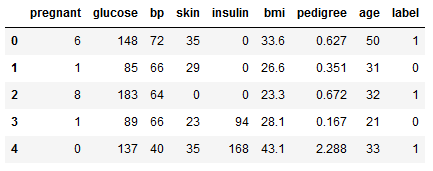
\includegraphics[width=0.6\linewidth,keepaspectratio]{pima1}
% \end{center}
% \end{frame}

% %%%%%%%%%%%%%%%%%%%%%%%%%%%%%%%%%%%%%%%%%%%%%%%%%%%%%%%%%%%
% \begin{frame}[fragile]\frametitle{Training}
% \begin{lstlisting}
% X = pima.drop('label', axis=1)
% y = pima.label

% from sklearn.cross_validation import train_test_split
% from sklearn.naive_bayes import MultinomialNB, GaussianNB
% from sklearn import metrics

% X_train, X_test, y_train, y_test = train_test_split(X, y, random_state=1)

% # testing accuracy of Multinomial Naive Bayes
% mnb = MultinomialNB()
% mnb.fit(X_train, y_train)
% y_pred_class = mnb.predict(X_test)
% print(metrics.accuracy_score(y_test, y_pred_class)) #0.54166

% # testing accuracy of Gaussian Naive Bayes
% gnb = GaussianNB()
% gnb.fit(X_train, y_train)
% y_pred_class = gnb.predict(X_test)
% print(metrics.accuracy_score(y_test, y_pred_class)) # 0.7916
% \end{lstlisting}
% \end{frame}

% %%%%%%%%%%%%%%%%%%%%%%%%%%%%%%%%%%%%%%%%%%%%%%%%%%%%%%%%%%%
% \begin{frame}[fragile]\frametitle{Conclusion}
% \begin{itemize}
% \item When applying Naive Bayes classification to a data-set with continuous features, it is better to use Gaussian Naive Bayes than Multinomial Naive Bayes.
% \item  The latter is suitable for data-sets containing discrete features (e.g., word counts).
% \end{itemize}
% \end{frame}